Dans un derniers effort nous avons poussée notre simulation vers les haut nombres de Reynolds, nous avons pu observer des 
comportements chaotiques. Là encore nos visualisation nous on permis de quantifier ce comportement.

\begin{figure}[hbtp]
  \centering
  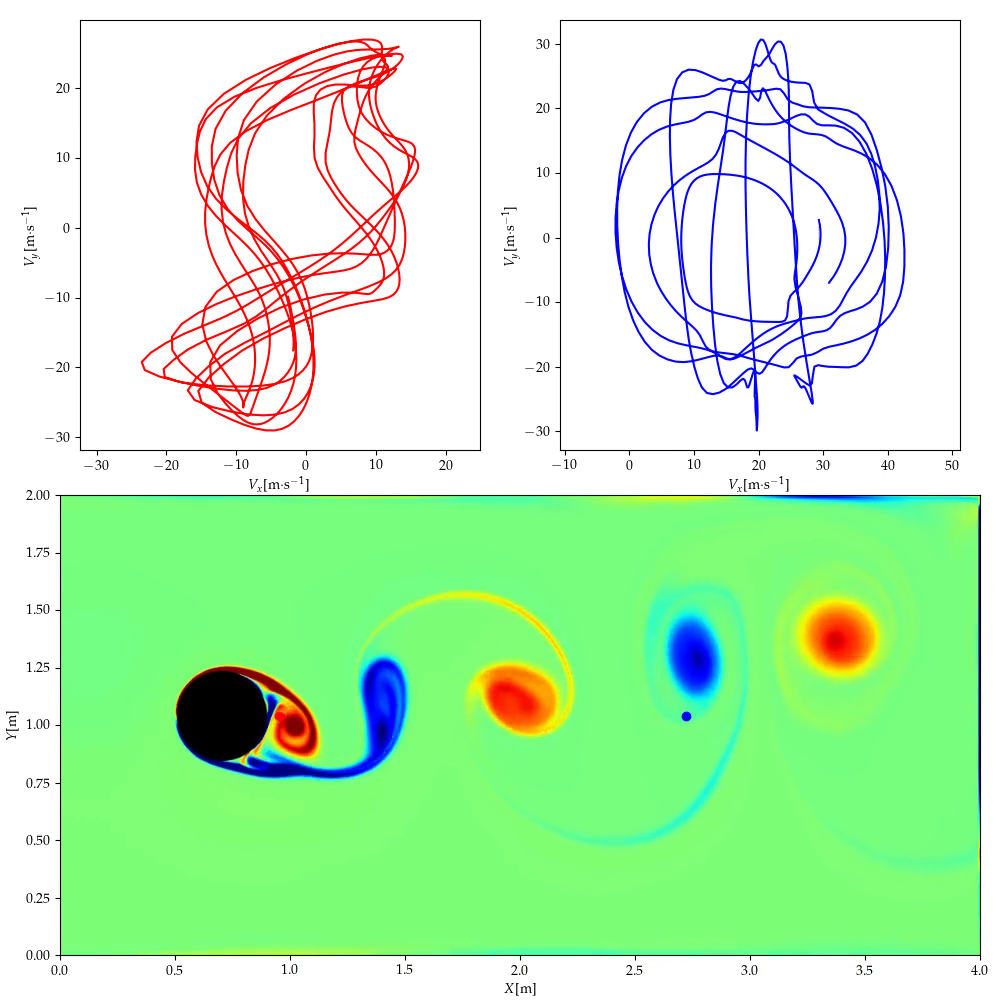
\includegraphics[width=\linewidth]{Fig/little_chaos.png}
  \caption{Rotationnel d'un écoulement chaotique $Re \approx 1000$}
  \label{fig:lChaos}
\end{figure}

Les comportements chaotiques sont très riches et nous aurions aimé plus étudier ces simulation malheureusement ces simulations arrievent à la limite de ce qui est faisable techniquement avec le matériel à notre disposition.\footnote{les simulations des figures \ref{fig:lChaos} et \ref{fig:VK} on nécessité chacune plus de 120 Go de stockage et plus de 6h de simulations.}
\begin{figure}[hbtp]
  \centering
  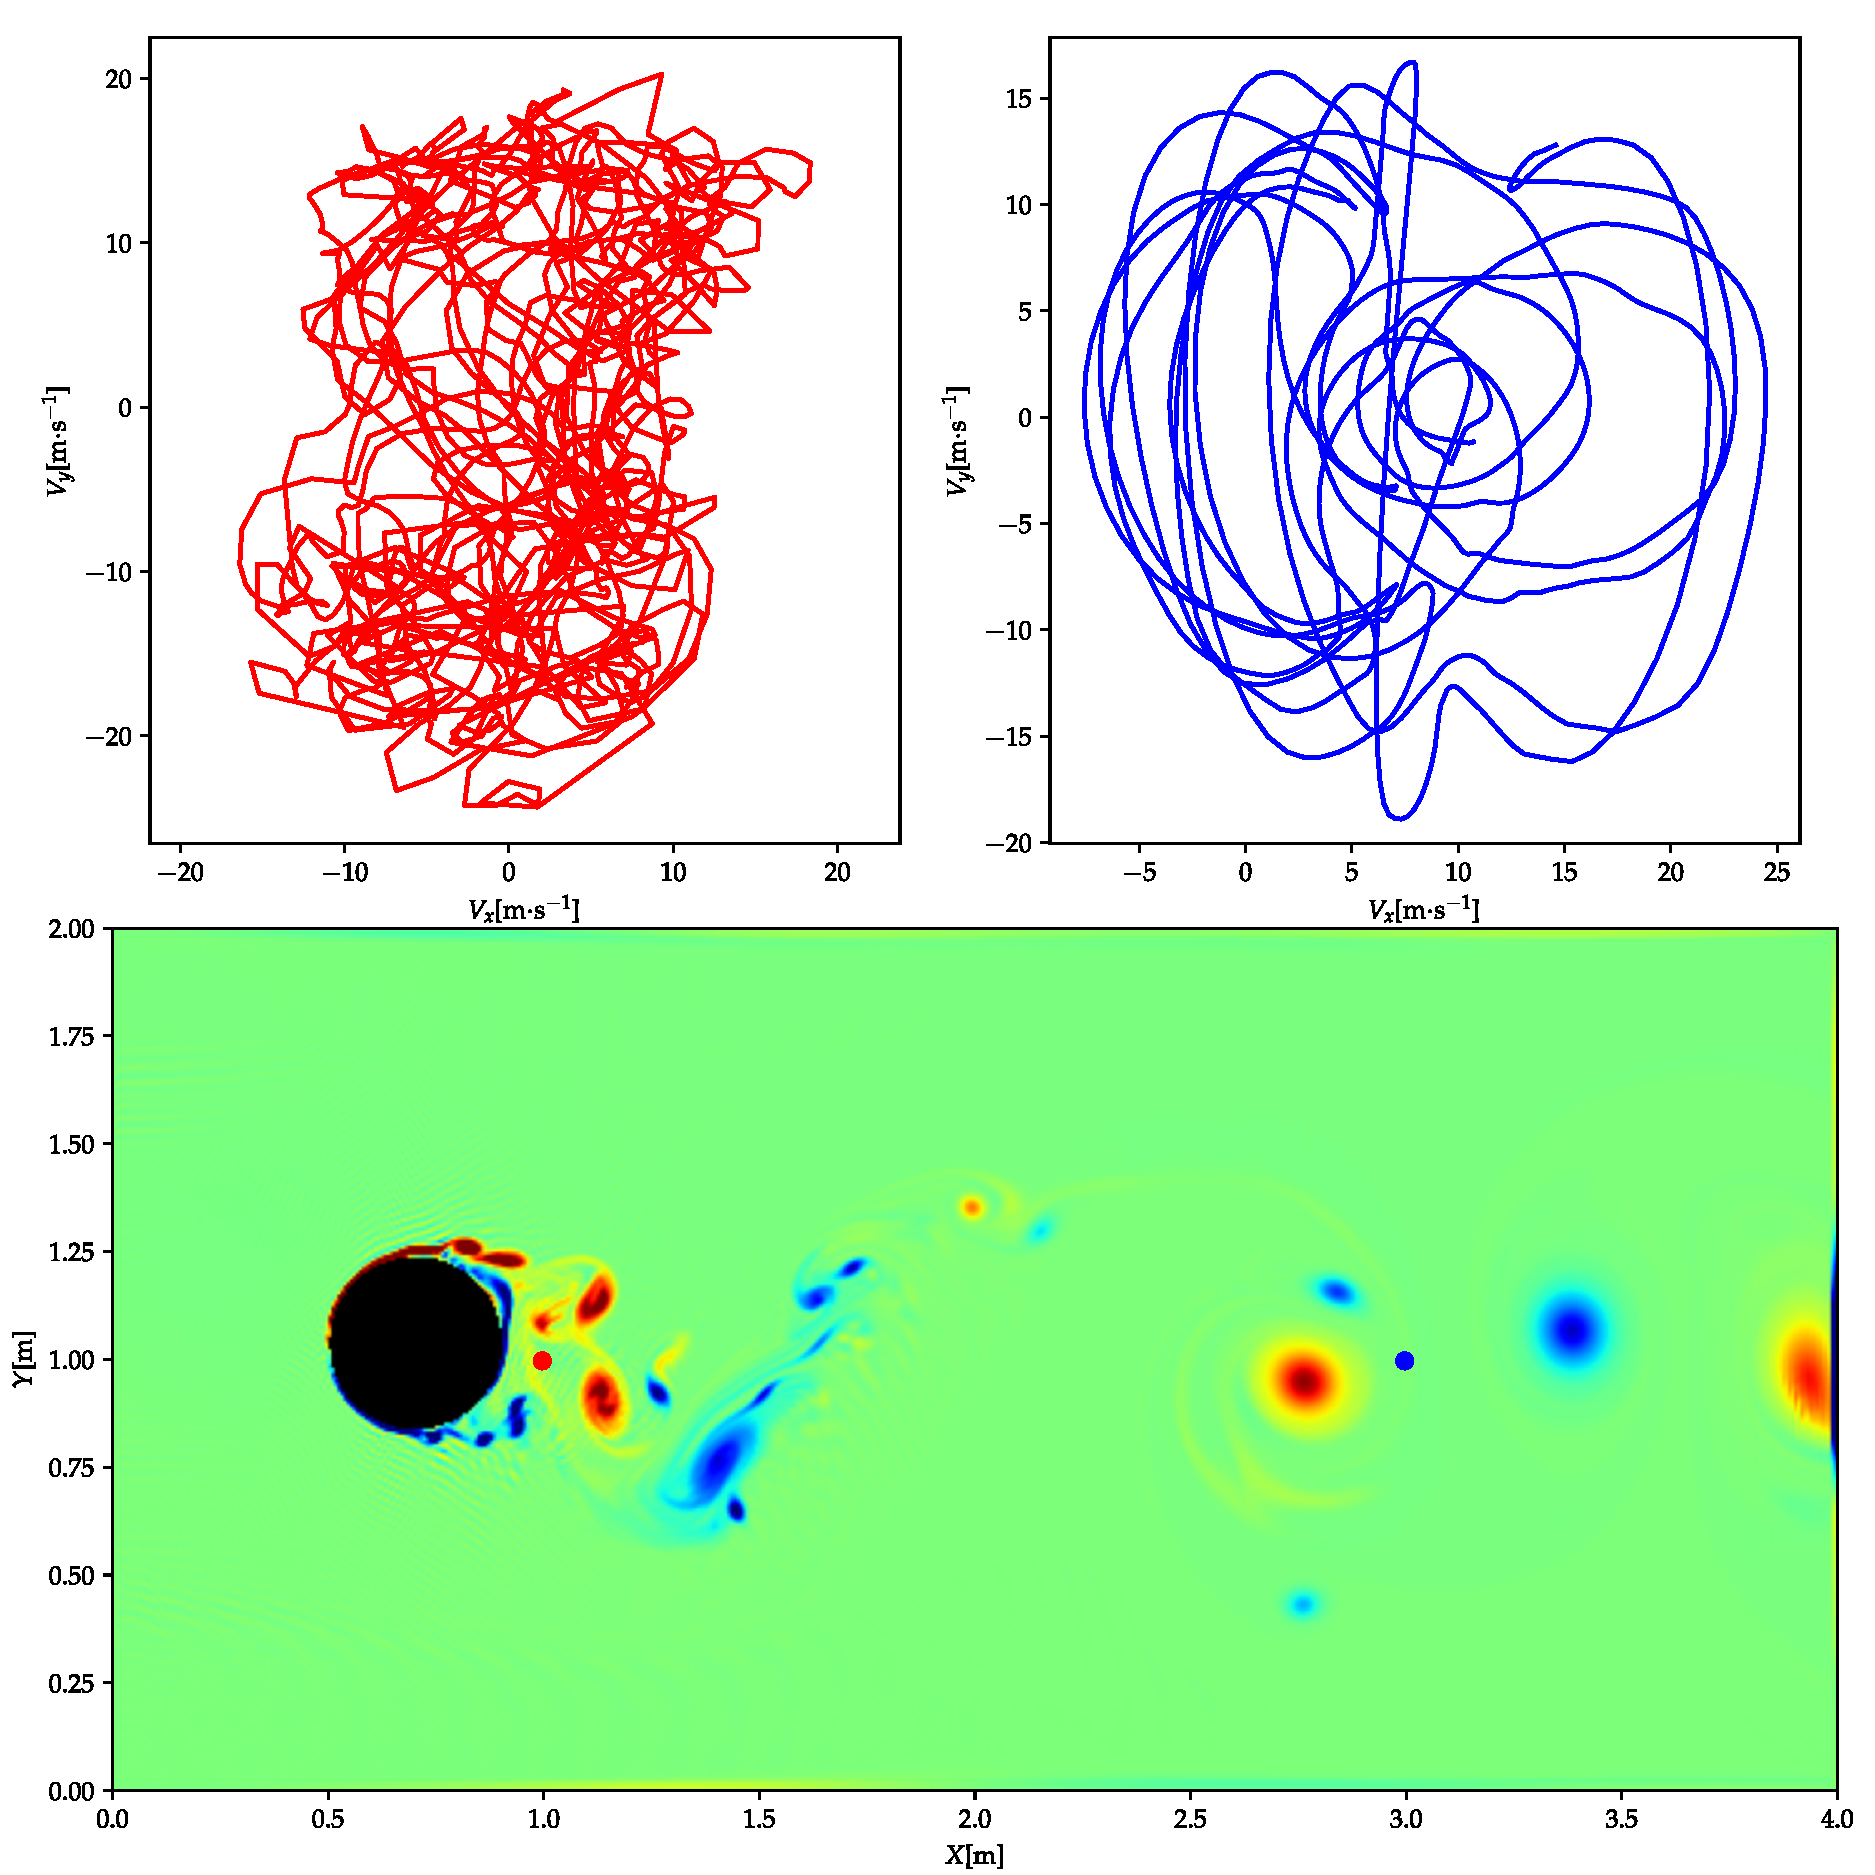
\includegraphics[width=\linewidth]{Fig/chaos.pdf}
  \caption{Rotationnel d'un écoulement chaotique $Re \approx 4000$}
  \label{fig:Chaos}
\end{figure}